\begin{IEEEbiography}[{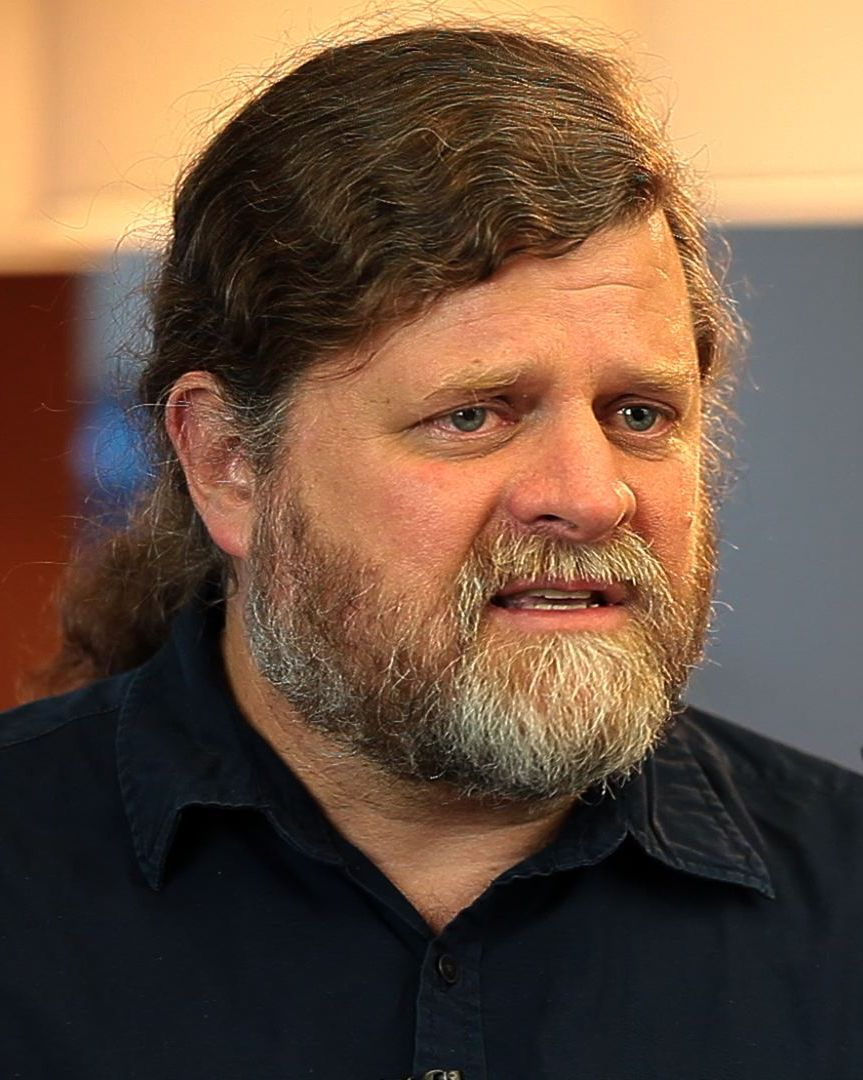
\includegraphics[width=1in,height=1.25in,clip,keepaspectratio]{tim}}]{Timothy G. Mattson}
received a PhD degree in chemistry (UCSC1985). 
He leads the Programming Systems Research group at Intel
where he works on parallel programming models,
Graph algorithms in terms of  sparse linear algebra, polystore data management systems,
and machine learning applied to software generation. 
He was part of the original crew that created OpenMP back in 1996
and served as one of the first CEOs of the OpenMP ARB.   
\end{IEEEbiography}

